\section{Numerical Results}
\label{sec:numRes}
We now have some MFT predictions about the SPM, and a few ideas about when those predictions might be invalid. Thus, it is prudent for us to test them out numerically.
There are a few different methods which could have been used, but we chose to calculate using the excellent \texttt{KMCLib}\cite{leetmaa2014kmclib} package, which implements the Kinetic Monte Carlo algorithm (essentially the same as the Gillespie algorithm)
on lattice systems. \texttt{KMCLib} has the advantage that it is python-wrapped \texttt{C++}, and thus quite easy to use whilst at the same time being quite computationally efficient; thus it was fairly easy for us to carry out large numbers
of differently-parametrised serial \texttt{KMCLib} jobs on the \texttt{Eddie3} computing cluster here at Edinburgh. The codes used are kept here~\cite{jHellGitRepo}.
\subsection{Flow in a Block}
As we have MFT predictions about flow in a block, we can try to simulate that situation using KMC. In the bulk, the transition rates are simply those described in Figure~\ref{fig:rates}. At the boundaries, referred to as the ``top'' and ``bottom''
of the block, there are 2 layers of lattice sites what switch between being full and empty with rates such that the time-averaged occupation can be specified to match the desired boundary conditions; there are then chances for particles to spawn
and despawn with rates depending upon the occupation of these boundary layers. In the end, the intention is that these boundaries should reproduce the effect of having particle reservoirs attached to the ends, which is something we can check for
sanity in the output by inspecting the time-averaged occupations of sites near the boundary.

In our calculations, we set the top and bottom densities to be $\rho_T = \rho_M - \frac{1}{2} \delta\rho$ and $\rho_B = \rho_M + \frac{1}{2} \delta\rho$ respectively, as well as specifying the value of $\lambda$ and the number of sites
in the lattice. During the calculation, we perform a specified number
of Gillespie steps, and count the number of particles entering at the top $e_T$, leaving at the top $l_T$, entering at the bottom $e_B$, leaving at the bottom $l_B$, as well as the Gillespie time interval $T$ that elapses during
those steps; we then have an estimate of the overall flow rate $J$ via
\begin{equation}
 J = \frac{e_B-e_T+l_T-l_B}{2T}.
\end{equation}
We can also count the total number of particles in the system in order to measure the average particle density, although we need to make sure that it is correctly time-averaged.
If we keep $\delta\rho$ relatively small, $J$ varies approximately linearly with $\delta\rho$; thus if we calculate $J$ for a series of small $\delta \rho$, we can perform linear regression to find $D=\partDeriv{J}{\delta\rho}\big|_{\delta\rho=0}$,
the effective diffusion coefficient. Computing this for different $(\rho_M, \lambda)$ combinations gives us numerical data which can be compared with the MFT result in Equation~\ref{eq:MFTflow}.
\begin{figure*}[h!]
\vspace{1em}
\caption{\label{fig:diffCoef} The contour plot on the left shows the MFT prediction of the diffusion coefficient $D=\partDeriv{J}{\delta\rho}\big|_{\delta\rho=0}$ as a function of local density $\rho_M$ and $\lambda$;
we are only plotting where $0 \le D \le 1.2$, other regions are shown in white, including the region in which $D<0$, which would cause instabilities and so prevent a flow from actually occurring. On the right is our numerical calculation of $D(\rho_M, \lambda)$,
with exactly the same plotting ranges. The dots indicate which points in $(\rho_M, \lambda)$ we calculated $D$ around, to give an impression of how the interpolation in the contour plot was done.}
\begin{center}
 \begin{tabular}{c@{\hspace{1em}}c}
    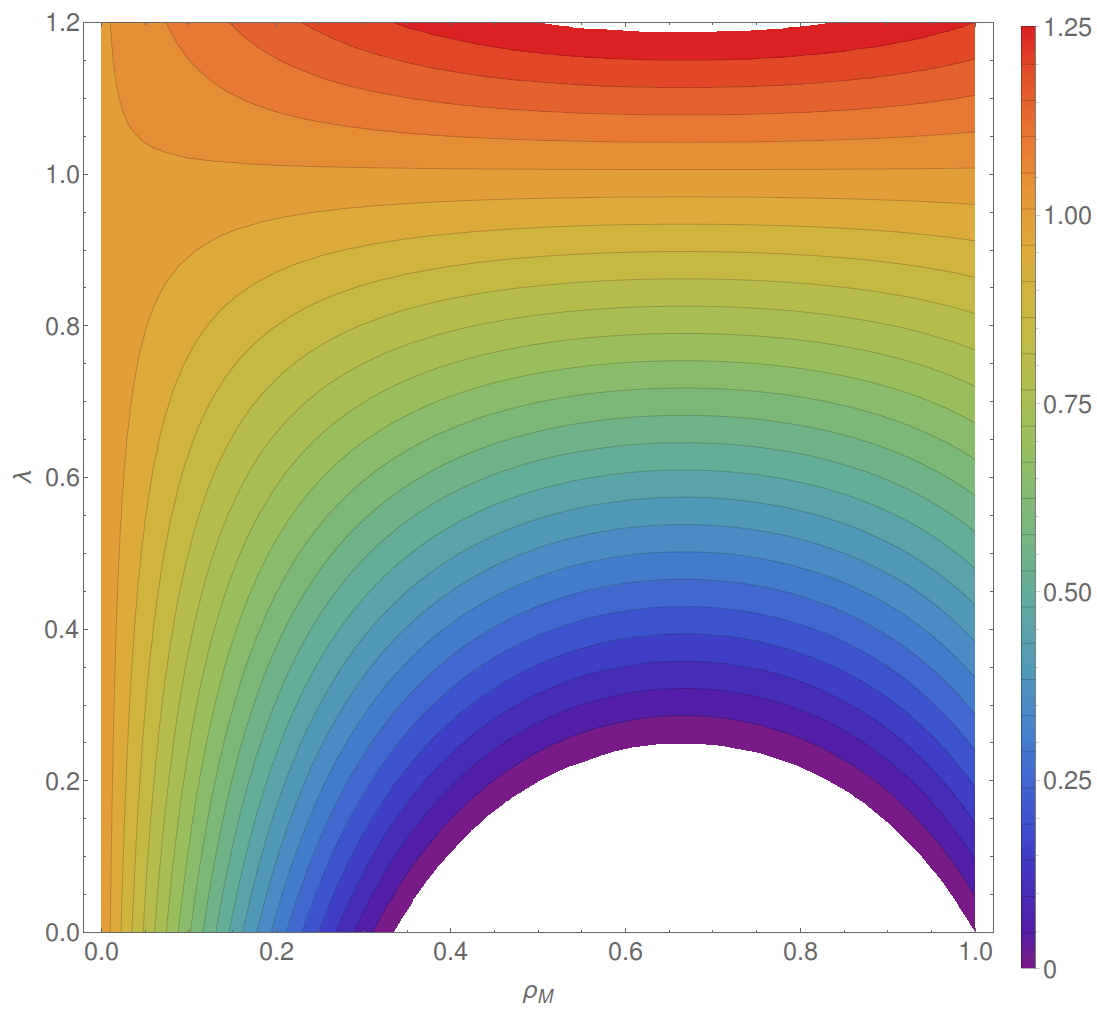
\includegraphics[width=0.5\linewidth]{../tex-src/images/analFlow.png} & 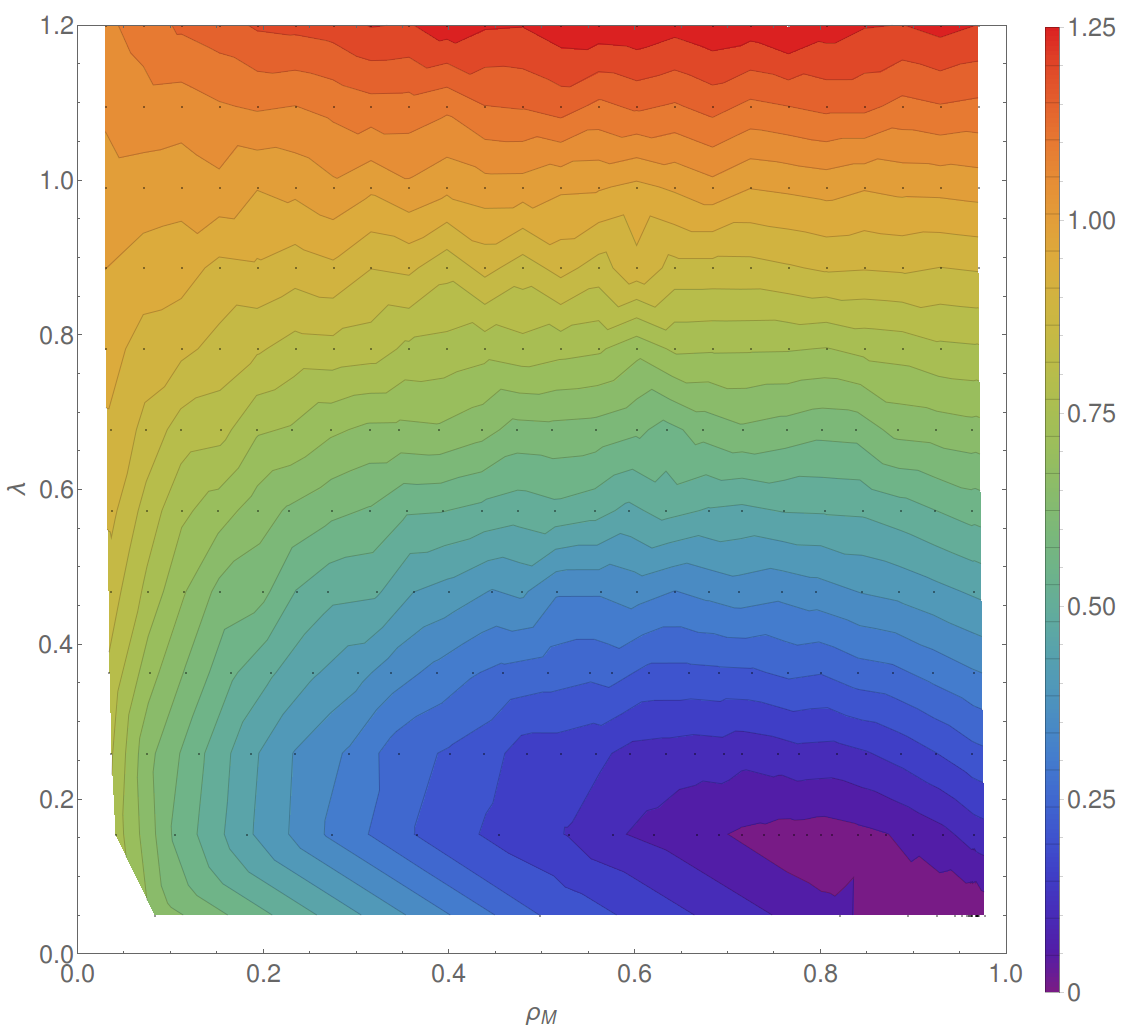
\includegraphics[width=0.5\linewidth]{../tex-src/images/dataFlow.png} \\
    \end{tabular}
\end{center}
    \vspace{-0em}
\end{figure*}
To produce the results in Figure~\ref{fig:diffCoef}, for each $(\rho_T, \rho_B, \lambda)$ combination we created the initial state by randomly inserting particles into an empty 124-length lattice, so that the density was $\rho_M$. We then ran the simulation for
$1.6\times10^8$ steps, to wash away any spurious initial-data effects and allow the system to reach a steady state flow. We then ran for $8\times10^7$ steps whilst measuring flow rate and density, then allowed the system to run for $1.6\times10^7$
steps without taking measurements in an effort to suppress temporal autocorrelation effects. This alternating process was repeated 10 times, yielding 10 measurements of flow rate and density, from which estimates of these quantities and their
standard errors could be obtained. The whole setup was repeated with a 60-length system, in order to check for edge effects; however, the results were not significantly different, so those would not seem to be a problem.

We can of course obtain estimates of the confidence interval for our linear regression coefficient, and thus generate a standard error for $D$; likewise we can obtain goodness of fit estimates for the
regression. They are not included here due to space constraints, but they are in the additional materials.
%REMEMBER TO ACTUALLY PUT IT THERE!!!

\subsection{Flow Structure}
\label{sec:flowStruc}
It is possible to produce diagrams which show the changes in short-time-averaged local density as a function of space and time. I have made such diagrams for a selection of $(\rho_M, \lambda)$ pairs, so that the reader can
get an impression of what these flows actually look like; they are shown in Figure~\ref{fig:flowPatterns}.
\iffalse
\begin{figure*}[h!]
\caption{\label{fig:flowPatterns} The spacetime flow patterns, for the $(\lambda, \rho_M)$ combinations indicated in the row and column headers. In each plot time runs along the $x$-axis, space along the $y$-axis. White represents full occupation, black empty, and grey shades partial
occupation. The degree of occupation was calculated by taking the \texttt{KMCLib} record of a particular site's occupation (i.e. the Gillespie times at
which the site changed occupation), assigning $0$ and $1$ to particles and vacancies respectively, linearly interpolating this and then integrating over times longer than a single Gillespie step but much shorter than the total time in question.
In each case the total time elapsed is that taken by $10^6$ Gillespie steps, and each short-time-average has been done over the total time divided by $508$ (to produce square diagrams, as there are $508$ active sites
per simulation). I chose to rescale time this way because if we used equal times it would appear that nothing happens in the low-$\lambda$ simulations, which isn't true!}
\begin{tabular}{c p{0.175\linewidth}}
\hspace{-2em}\begin{tabular}{c|c@{\hspace{0.25em}}c@{\hspace{0.25em}}c@{\hspace{0.25em}}c  }
  &  $\lambda=0.05$ & $\lambda=0.25$ & $\lambda=0.50$ & $\lambda=0.70$ \\ 
  \hline
   \begin{tabular}{c} \vspace{-12em} \\ \hspace{-1em}$\rho_M=0.05$\hspace{0em} \\  \\ \end{tabular} & 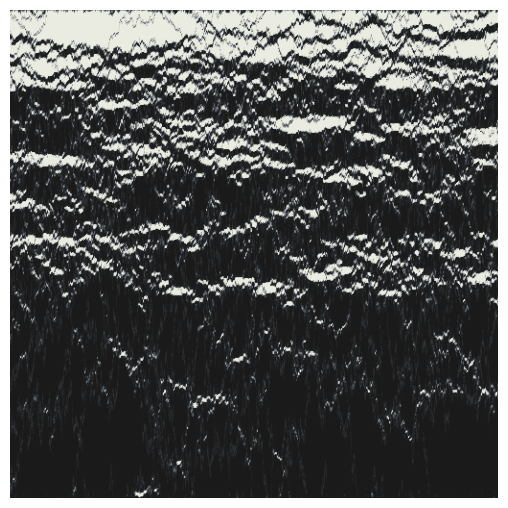
\includegraphics[width=0.24\linewidth]{../tex-src/images/flowImps/flowl0r0.png} & 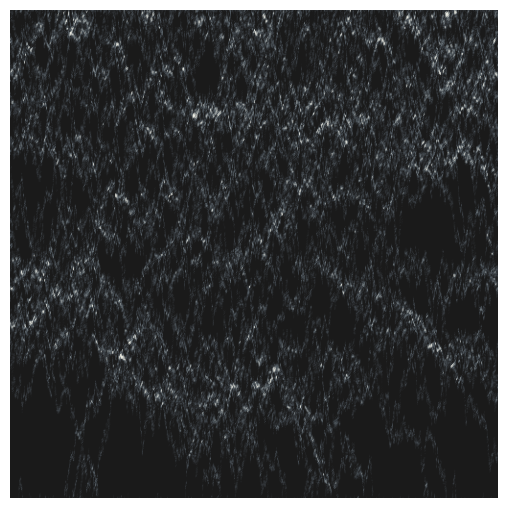
\includegraphics[width=0.24\linewidth]{../tex-src/images/flowImps/flowl1r0.png}  & 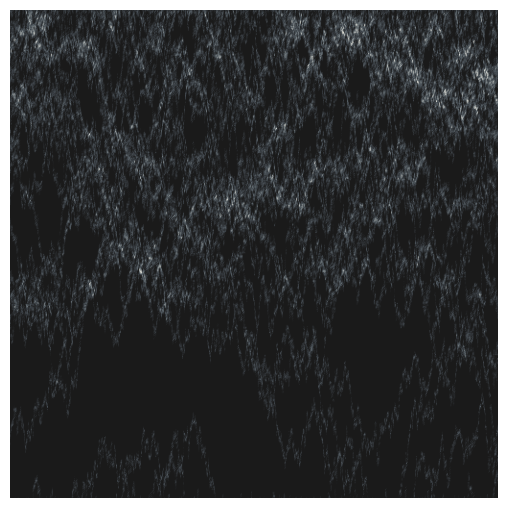
\includegraphics[width=0.24\linewidth]{../tex-src/images/flowImps/flowl2r0.png} & 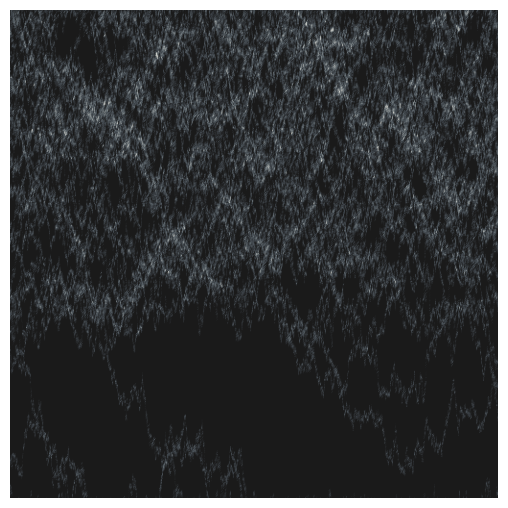
\includegraphics[width=0.24\linewidth]{../tex-src/images/flowImps/flowl3r0.png} \\
   \begin{tabular}{c} \vspace{-12em} \\ \hspace{-1em}$\rho_M=0.35$\hspace{0em} \\  \\ \end{tabular} & 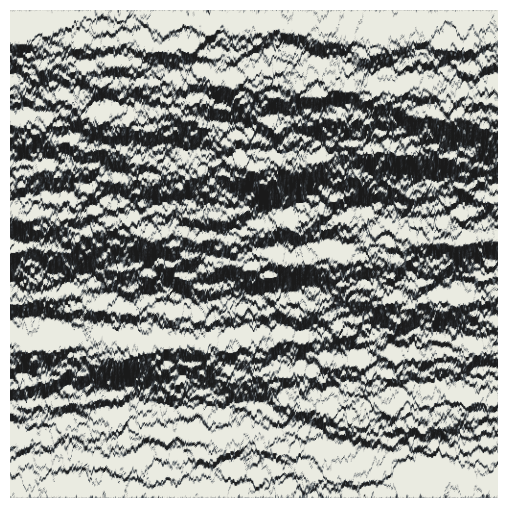
\includegraphics[width=0.24\linewidth]{../tex-src/images/flowImps/flowl0r1.png} & 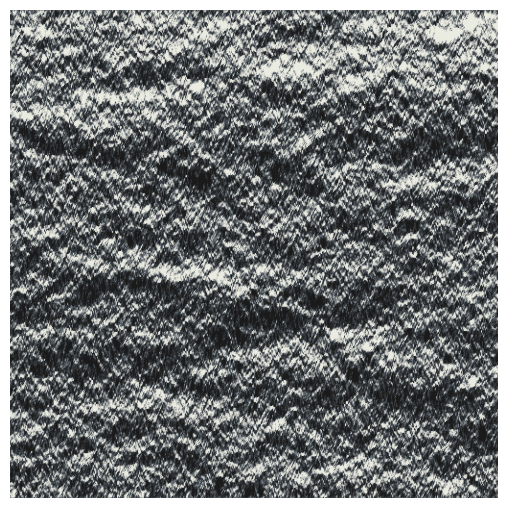
\includegraphics[width=0.24\linewidth]{../tex-src/images/flowImps/flowl1r1.png}  & 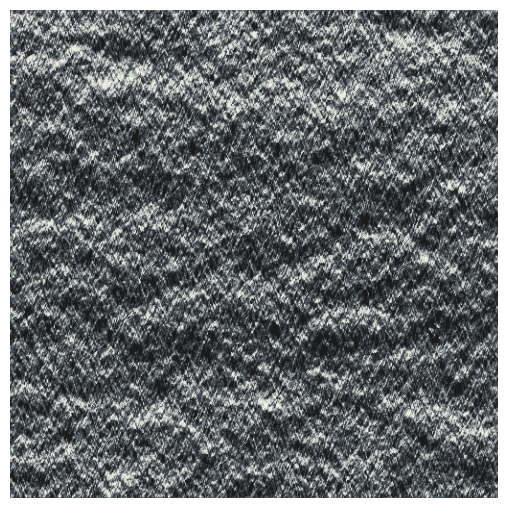
\includegraphics[width=0.24\linewidth]{../tex-src/images/flowImps/flowl2r1.png} & 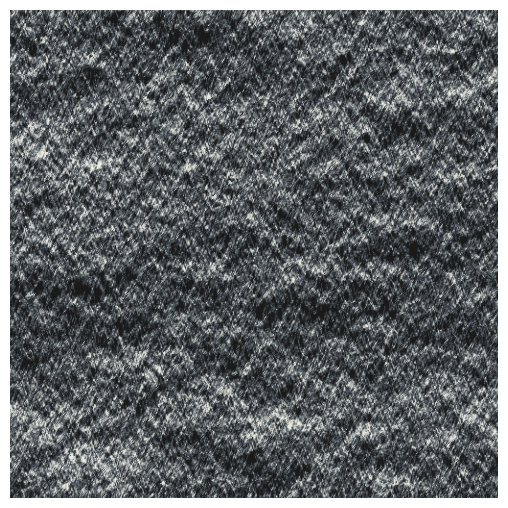
\includegraphics[width=0.24\linewidth]{../tex-src/images/flowImps/flowl3r1.png} \\
   \begin{tabular}{c} \vspace{-12em} \\ \hspace{-1em}$\rho_M=0.65$\hspace{0em} \\  \\ \end{tabular} & 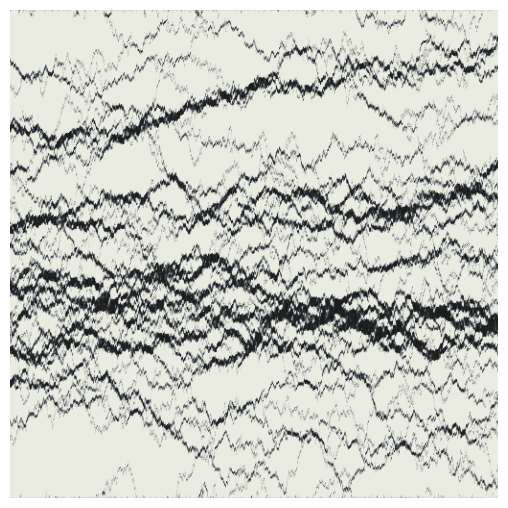
\includegraphics[width=0.24\linewidth]{../tex-src/images/flowImps/flowl0r2.png} & 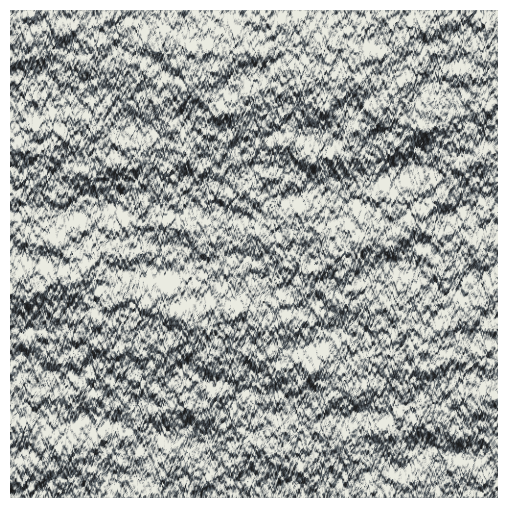
\includegraphics[width=0.24\linewidth]{../tex-src/images/flowImps/flowl1r2.png}  & 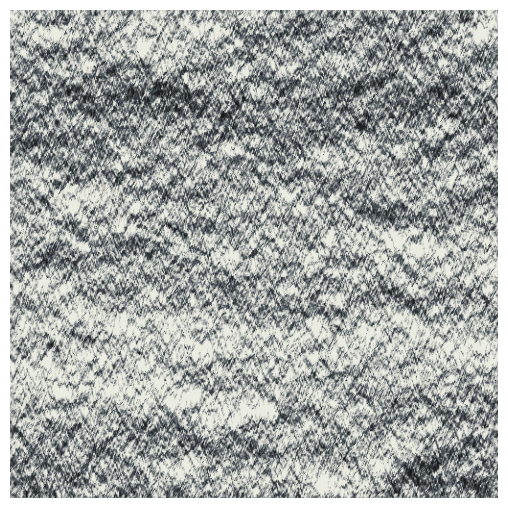
\includegraphics[width=0.24\linewidth]{../tex-src/images/flowImps/flowl2r2.png} & 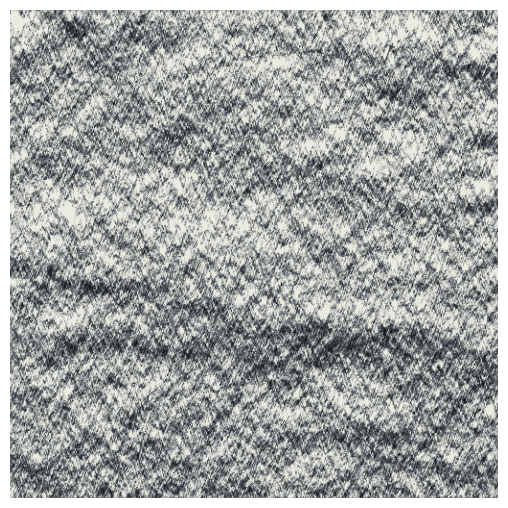
\includegraphics[width=0.24\linewidth]{../tex-src/images/flowImps/flowl3r2.png} \\
   \begin{tabular}{c} \vspace{-12em} \\ \hspace{-1em}$\rho_M=0.95$\hspace{0em} \\  \\ \end{tabular} & 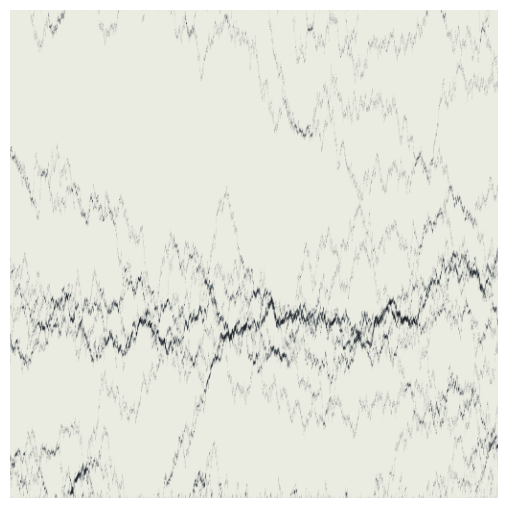
\includegraphics[width=0.24\linewidth]{../tex-src/images/flowImps/flowl0r3.png} & 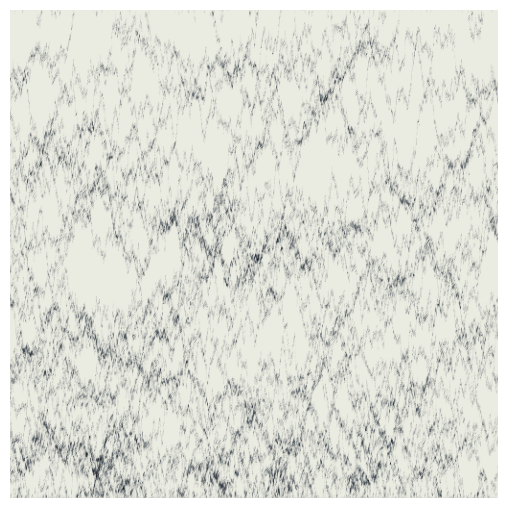
\includegraphics[width=0.24\linewidth]{../tex-src/images/flowImps/flowl1r3.png}  & 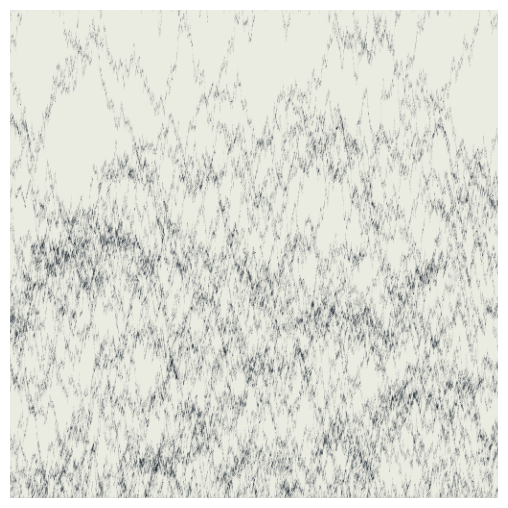
\includegraphics[width=0.24\linewidth]{../tex-src/images/flowImps/flowl2r3.png} & 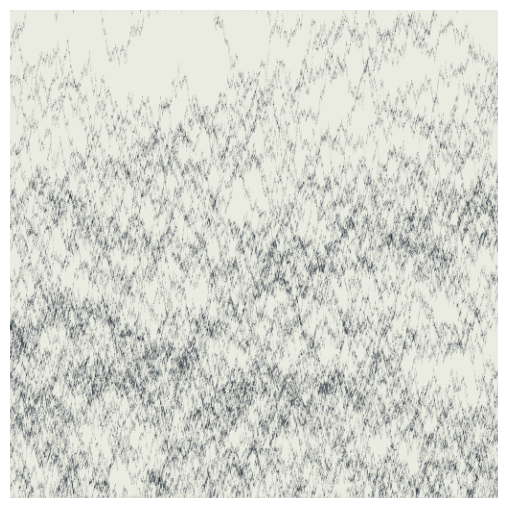
\includegraphics[width=0.24\linewidth]{../tex-src/images/flowImps/flowl3r3.png} \\
   \end{tabular}
\hspace{-1em}
&
\end{tabular}
\end{figure*}
\fi
\begin{figure*}[h!]
\caption{\label{fig:flowPatterns} The spacetime flow patterns, for the $(\lambda, \rho_M)$ combinations indicated in the row and column headers. In each plot time runs along the $x$-axis, space along the $y$-axis. White represents full occupation, black empty, and grey shades partial
occupation. The degree of occupation was calculated by taking the \texttt{KMCLib} record of a particular site's occupation (i.e. the Gillespie times at
which the site changed occupation), assigning $0$ and $1$ to particles and vacancies respectively, linearly interpolating this and then integrating over times longer than a single Gillespie step but much shorter than the total time in question.
In each case the total time elapsed is that taken by $10^6$ Gillespie steps, and each short-time-average has been done over the total time divided by $508$ (to produce square diagrams, as there are $508$ active sites
per simulation). Time has been rescaled this way in order to allow fair comparison of radically different $\lambda$-values.}
\begin{tabular}{c p{0.175\linewidth}}
\hspace{-2em}\begin{tabular}{c|c@{\hspace{0.25em}}c@{\hspace{0.25em}}c}
  &  $\lambda=0.05$ & $\lambda=0.38$ & $\lambda=1.00$ \\ 
  \hline
   \begin{tabular}{c} \vspace{-12em} \\ \hspace{-1em}$\rho_M=0.05$\hspace{0em} \\  \\ \end{tabular} & 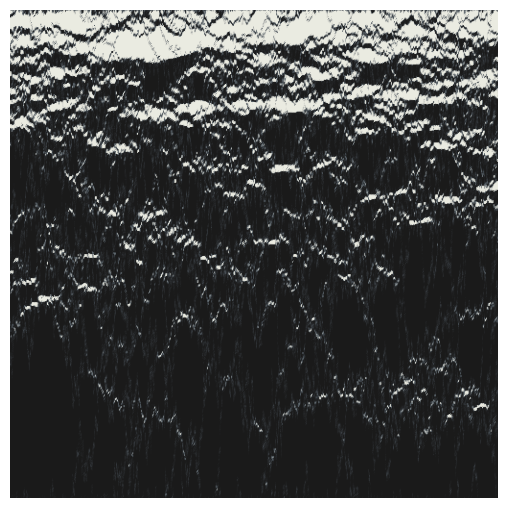
\includegraphics[width=0.32\linewidth]{../tex-src/images/flowImps2/flowl0r0.png} & 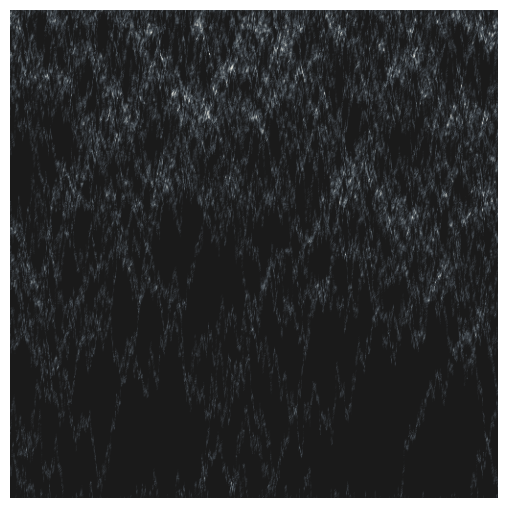
\includegraphics[width=0.32\linewidth]{../tex-src/images/flowImps2/flowl2r0.png}  & 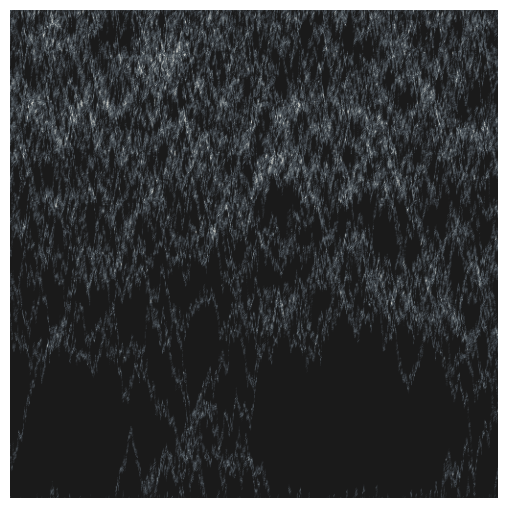
\includegraphics[width=0.32\linewidth]{../tex-src/images/flowImps3/flowl0r0.png} \\
   \begin{tabular}{c} \vspace{-12em} \\ \hspace{-1em}$\rho_M=0.50$\hspace{0em} \\  \\ \end{tabular} & 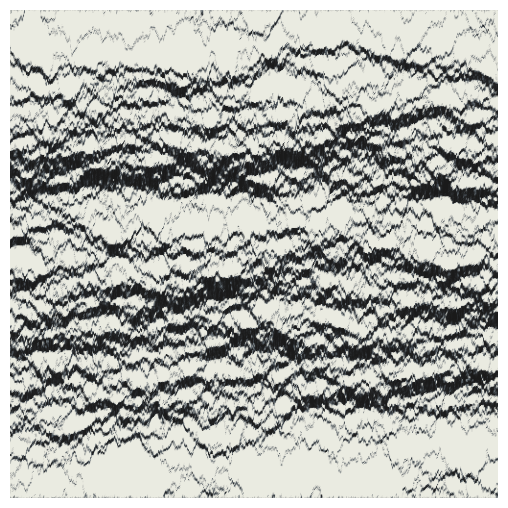
\includegraphics[width=0.32\linewidth]{../tex-src/images/flowImps2/flowl0r2.png} & 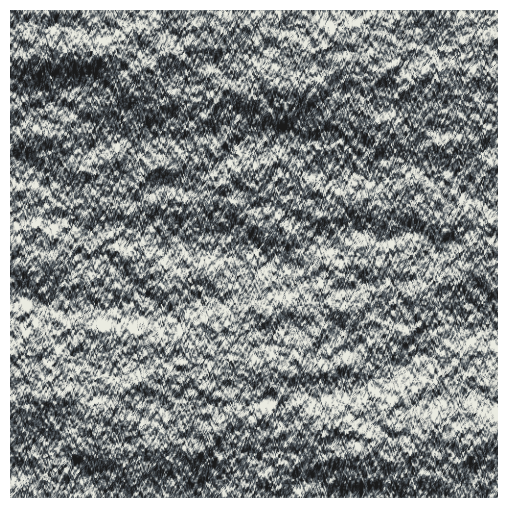
\includegraphics[width=0.32\linewidth]{../tex-src/images/flowImps2/flowl2r2.png}  & 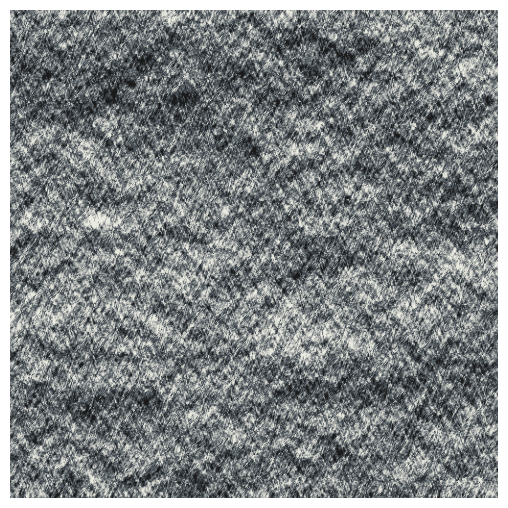
\includegraphics[width=0.32\linewidth]{../tex-src/images/flowImps3/flowl0r2.png} \\
   \begin{tabular}{c} \vspace{-12em} \\ \hspace{-1em}$\rho_M=0.95$\hspace{0em} \\  \\ \end{tabular} & 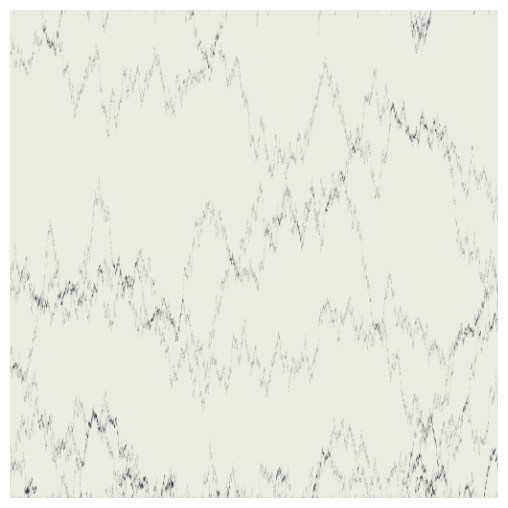
\includegraphics[width=0.32\linewidth]{../tex-src/images/flowImps2/flowl0r4.png} & 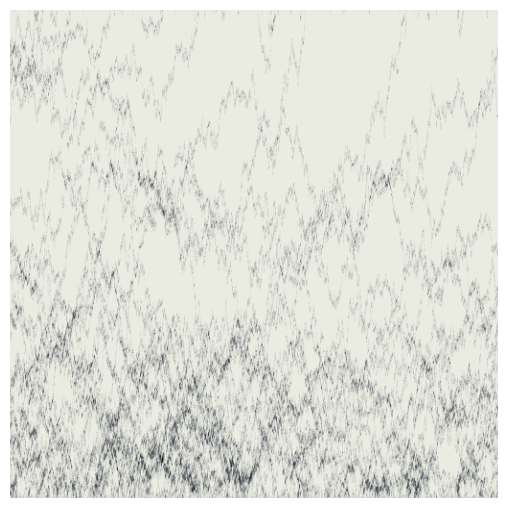
\includegraphics[width=0.32\linewidth]{../tex-src/images/flowImps2/flowl2r4.png}  & 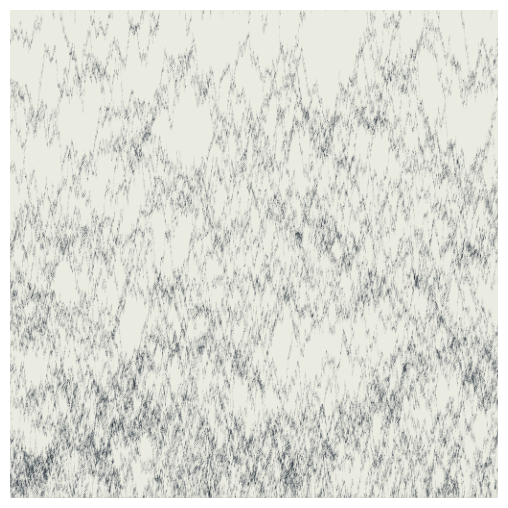
\includegraphics[width=0.32\linewidth]{../tex-src/images/flowImps3/flowl0r4.png} \\
   \end{tabular}
\hspace{-1em}
&
\end{tabular}
\end{figure*}

\iffalse
\subsection{Correlation Functions}
Whilst we're calculating flow rates, we can also use our \texttt{KMCLib} code to calculate the equal time 2-point correlation function
$C(x) = \left\langle \rho(x)\rho(0) \right\rangle - \left\langle \rho(x) \right\rangle \left\langle \rho(0) \right\rangle $.
We can calculate the same quantity in a finite periodic ring analytically, and in both the analytic and numerical cases we may attempt to extract a correlation length by (curve-fitting / Laplace transform);
hence we can check whether having a steady flow through the system causes any structural effects.}
\fi